\documentclass[a4paper]{article}
\usepackage[UTF8]{ctex}
\usepackage{tikz}
\usepackage{xcolor}
\usepackage{amsmath}
\usepackage{amsthm}
\usepackage{amssymb}
\usepackage{enumerate}
\usepackage{float}
\usepackage{arydshln}
\usepackage{listingsutf8}
\usepackage{listings-ext}
\usepackage[margin=1in]{geometry}
% https://www.latexstudio.net/archives/9774.html
% https://www.latexstudio.net/archives/2234
% https://texample.net/

\lstset{
    basicstyle=\tt,
    keywordstyle=\color{purple}\bfseries,
    identifierstyle=\color{brown!80!black},
    commentstyle=\color{gray}
    showstringspaces=false,
    breaklines=true % 自动换行
}

\newtheorem{theorem}{\indent 定理}[section]
\newtheorem{lemma}[theorem]{\indent 引理}
\newtheorem{proposition}[theorem]{\indent 命题}
\newtheorem{corollary}[theorem]{\indent 推论}
\newtheorem{definition}{\indent 定义}[section]
\newtheorem{example}{\indent 例}[section]
\newtheorem{remark}{\indent 注}[section]
\newenvironment{solution}{\begin{proof}[\indent\bf 解]}{\end{proof}}
\renewcommand{\proofname}{\indent\bf 证明}

\tikzset{eaxis/.style={->,>=stealth}}

\title{组合优化与凸优化作业3}

\author{HOMODELUNA}
\date{2025 年 5 月 5 日}

\begin{document}
\maketitle
\section{}
结合具体的最优化方法来解释优化中的迭代与逼近思想。

\paragraph{答}
在优化问题中,迭代与逼近思想是核心概念。通过不断更新解的估计,我们可以逐步逼近最优解。下面将以梯度下降法和共轭梯度法为例进行详细说明。

\subsection{梯度下降法}

梯度下降法是一种基于一阶导数的信息来寻找函数局部最小值的迭代方法。其基本思想是:

1. 从一个初始点 \( x_0 \) 开始。
2. 计算该点的梯度 \( \nabla f(x_k) \)。
3. 沿着梯度的反方向更新当前点:
   \[
   x_{k+1} = x_k - \alpha \nabla f(x_k)
   \]
   其中,\( \alpha \) 是学习率,控制每次迭代的步长。

通过不断迭代这一过程,\( x_k \) 会逐步逼近函数的最小值。梯度下降法的一个关键问题是选择合适的学习率,过大可能导致不收敛,过小则收敛速度慢。

\subsection{共轭梯度法}

共轭梯度法是一种用于求解大型线性系统和二次优化问题的有效迭代方法。与梯度下降法不同,共轭梯度法不仅考虑当前点的梯度,还利用之前的迭代信息,从而加速收敛。

其基本步骤如下:

1. 初始化 \( x_0 \) 和残差 \( r_0 = b - Ax_0 \),以及初始搜索方向 \( p_0 = r_0 \)。
2. 在每次迭代中,计算步长 \( \alpha_k \):
   \[
   \alpha_k = \frac{r_k^T r_k}{p_k^T Ap_k}
   \]
3. 更新当前解:
   \[
   x_{k+1} = x_k + \alpha_k p_k
   \]
4. 更新残差:
   \[
   r_{k+1} = r_k - \alpha_k Ap_k
   \]
5. 计算新的搜索方向:
   \[
   \beta_k = \frac{r_{k+1}^T r_{k+1}}{r_k^T r_k}
   \]
   \[
   p_{k+1} = r_{k+1} + \beta_k p_k
   \]

通过这一过程,共轭梯度法能够在较少的迭代次数内收敛,特别适用于大规模问题。

\subsection{总结}

无论是梯度下降法还是共轭梯度法,迭代与逼近的思想都是通过反复更新解的估计来接近最优解。这种方法在实际应用中非常有效,尤其是在高维空间和复杂优化问题中。
\section{}
假设优化问题为\(\min f(x)\);s,t. $g(x) \leq 0,h(x) = 0$,其中$f: \mathbb{R}^n \rightarrow \mathbb{R}$,$g : \mathbb{R} \rightarrow \mathbb{R}$, $h : \mathbb{R} \rightarrow \mathbb{R}$,假
设在点$x_k \in \mathbb{R} ^n$处,方向 $d \in \mathbb{R}^n$是该点处的某个方向,若该方向是可行下降方向,请推导方
向$d$必须满足的条件。 

\paragraph{解}

\[\left\{\begin{array}{c}
    \nabla f(x_k) \cdot d \leq 0 \\
    \nabla h(x_k) \cdot d  = 0\\
    \nabla g(x_k) \cdot d \leq 0 \quad or \quad g(x_k) > 0 
\end{array}\right.\]

\section{}

用最速下降法求解 \(\min f(x) = x_1 - x_2 + 2x_1^2 +2x_1x_2 +x_2^2\),取\(x_0 = (0,0)^T\)要求迭代两次。

\paragraph{解}

对原函数求梯度, \(g(x) = [1+4x_1 + 2x_2, -1 +2x_2 + 2x_1]\) ,取迭代步长为$d=0.1$, 有

\[g(x_0) =(1,-1)^T \]

此时 \(\phi(d) =d^{2} + 2 d\) 当\(d = -1\)时取最小值,此时$x = (-1,1)$

在$x= (-1,1)$上,$g(x) = (-1,-1)$,此时\(\phi(d) = 5 d^{2} + 2 d - 1\),当$d=-0.1$时取最小值.此时$x=(-0.9,1.1)$


\section{}

考虑下述问题 \[\min f(x) = 2x_1^2 + 2x_2^2 -2x_1x_2 -4x_1 - 6x_2, \quad s.t. \quad \left\{\begin{array}{c}
    x_1 + x_2 \leq 2 \\
    x_1 + 5x_2 \leq 5 \\
    -x_1 \leq 0 \\
    -x_2 \leq 0 \\
\end{array}\right.\]

\subsection{}

试求目标函数$f(x)$的梯度,以及临界点和Hessian矩阵$H$,并判定各临界点是否是真正的极值点。

梯度 $g(x) = (4x_1 -2x_2 - 4,4x_2 -2x_1-6)$

hessian 矩阵 \(H(x) = \left(\begin{matrix}
    4 & -2\\
    -2 & 4
\end{matrix}\right)\)

目标函数的临界点为$(1,2)^T$,经验证,它不满足极值条件,因此不可能为极值点

\subsection{}

试求各约束条件的梯度.

\paragraph{解}
各约束条件分别为
\[\left\{\begin{array}{c}
    x_1 + x_2 \leq 2 \\
    x_1 + 5x_2 \leq 5 \\
    -x_1 \leq 0 \\
    -x_2 \leq 0 \\
\end{array}\right.\]

其梯度分别为:
\[\left\{
\begin{array}{c}
    g_1(x) = (1,1)^T \\
    g_2(x) = (1,5) ^T\\
    g_3(x)=(-1,0)^T \\
    g_4(x) = (0,-1)^T\\
\end{array}
\right\}\]

\subsection{}

假设从初始点$x(1) =(0,0)$ 出发,采用约束优化问题的可行方向法来求解该问题  

\paragraph{解}
在该点$(0,0)$的梯度为$g((0,0)^T)=(-4,-6)^T$,此时$g_3,g_4$处于临界状态,故可行方向的要求是:
\[\left\{
\begin{array}{c}
   d \cdot (-1,0)^T \leq 0\\
   d \cdot (0,-1)^T \leq 0\\
   \text{最小化} d \cdot (-4,-6)
\end{array}
\right\}\]

解得$d = (2,3)^T$,于是在该方向上$\phi(d) = 14d^2 - 26d$,此时考虑约束
\[\left[\begin{matrix}
   5 d - 2\leq 0\\17 d - 5\leq 0\\- 2 d\leq 0\\- 3 d \leq 0
\end{matrix}\right]\]

解得 $0 \leq d \leq \frac{5}{17}$

\(\phi(d)\)在$d= \frac{13}{14}$取最小值,但是该最小值不在约束条件内,最多可以取到$d=\frac{5}{17}$,此时$x = (\frac{10}{17},\frac{15}{17})$

此时$g_2: x_1 + 5x_2 \leq 5$为有效约束,函数梯度为\((- \frac{58}{17},- \frac{62}{17})^T\)
于是d的约束为
\[\left\{
\begin{array}{c}
   d \cdot (1,5)^T \leq 0\\
    \text{最小化} d \cdot (- \frac{58}{17},- \frac{62}{17})^T \leq 0\\
\end{array}
\right\}\]
解得合适的可行方向$d = (5,-1)$,此时$\phi(d) = 62 d^{2} - \frac{228 d}{17} - \frac{1860}{289}$,

$\phi(d)$在\(d = \frac{57}{527}\)处取最小值,此时 $x=(\frac{35}{31},\frac{24}{31})$,在该点,函数没有更多的可行方向.

\section{}
考虑约束最优化问题

\[\min f(x) = 4x_1^2 + x_2^2 +5x_1x_2 -4x_1 - 6x_2, \quad s.t. \quad \left\{\begin{array}{c}
    x_1^2 - x_2+2 \leq0 \\
    x_1 + x_2 -6 \leq 0 \\
    x_1 \geq 0 \\
    x_2 \geq 0 \\
\end{array}\right.\]
分别写出用内点法和外点法求解的辅助问题 .
\paragraph{解}


外点法(罚函数法):
\[\min f(x) + \mu \sum_{i=1}^{4}[\max(0,g_i(x))]^2, \quad s.t. \quad \left\{\begin{array}{c}
   g_1(x) = x_1^2 - x_2+2  \\
   g_2(x)= x_1 + x_2 -6 \\
   g_3(x)= x_1 \geq 0 \\
    g_4(x) = x_2 \geq 0 \\
\end{array}\right.\]

其中$\mu$为约束条件的惩罚系数,是一个很大的正数.

内点法(闸函数法):

\[\min f(x) + \mu B(x) \quad s.t. \quad x \in \mathbb{R}^n\]

其中:

\[B(x) = -\frac{1}{x_1^2-x_2 + 1} - \frac{1}{x_1 + x_2 - 6}+ frac{1}{x_1}+\frac{1}{x_2}\]

其中$\mu$为约束条件的惩罚系数.

注: 外点法的初始点选取不需要要求在可行域内部, 同时能够处理等式和不等式约束, 内点法仅适用于不等式约束,同时对初始点的选取有要求.

\section{}
给定如下的原问题(Primal Problem)和拉格朗日对偶问题(Lagrangian Duality Problem): 

\textbf{原问题}: \(\min_x f(x), s.t. \left\{ \begin{array}{cc}
   g_i(x) \leq 0 &, i = 1,...,m\\
   h_j(x)=0&,j=1,...,l\\
   x \in X &
\end{array}\right.\)其中$f,g_i,h_i : \mathbb{R}^n \rightarrow \mathbb{R}, X \subset \mathbb{R}^n$,为非空集合, 一般可令\(g = \left(\begin{matrix}
   g_1 \\ \vdots  \\ g_m
\end{matrix}\right)\), \(h = \left(\begin{matrix}
   h_1 \\ \vdots \\ h_l
\end{matrix}\right)\),来进一步优化表达式.

\textbf{对偶问题}: 
\(\max_{u,v}\theta(u,v),\quad s.t.\quad u \geq 0\),其中\(\theta(u,v) = \inf\{f(x)+\sum_{i=1}^m u_i g_i (x) + \sum^l_{j=1}v_j h_j(x) : x \in X\}\), \(u \in \mathbb{R}^m\),\(v \in \mathbb{R}^l\)分别表示对应不等式和等式约束的拉格朗日乘子向量和对偶变量.

\subsection{}
证明: 函数\(\theta(u,v)\)是凹函数.

\paragraph{证明}
首先考虑拉格朗日方程中 $L(x,u,v)$ 中,对于每一个固定的 $x$,$L(x,u,v)$ 对于 $(u,v)$ 都是仿
射的,根据仿射函数的性质(仿射函数即是凸的也是凹的),可以得到$L(x,u,v)$ 对 $(u,v)$ 是凹的.
 $\theta(u,v)$ 是对 $L(x,u,v)$ 取 pointwise infimum 的结果,所以 $\theta(u,v)$ 是凹的.

注:对于多个凸函数,我们知道 pointwise maximum 操作是保凸的. 对于多个凹函数,我们知道:pointwise infimum 操作保持凹性的.

\subsection{}
请解释对偶问题在最优化中的作用,简单论述弱对偶定理和强对偶定理的内容。

\paragraph{答}
对偶问题在最优化中的作用:通过(1)中的证明我们可以知道,一个优化问题的拉格朗日对偶问题一定是一个凹问题,这对于原问题的目标函数和不等式约束的凸性没有要求。同时,对偶的性质还保证的对偶问题的最优解一定是原问题的下界,即有$\theta(u,v)\leq p^*,\forall u\geq0, \forall v$,其中$p^*$ 是原问题的最优解,在弱对偶定理和强对偶定理的帮助下,可以很容易的估计原问题的最优解的界,甚至将原问题转换成对偶问题求解.

弱对偶定理: $\inf{f(x)|x \in S} \geq sup{\theta(u,v)}$
说明:即对偶问题的上界是原问题的下界,但是不等式的等号不一定能够取到.
强对偶定理:存在 $ \hat{x}$, 使得$\inf\{f( \hat{x})| \hat{x} \in S\} = \sup\{\theta(u,v)\}$

\section{}
给定优化问题 \(\min (x_1-3)^2+(x_2 -2)^2, \quad s.t. \quad \left\{\begin{array}{cl}
   x_1^2 + x_2^2 & \leq 5\\
   x_1 + 2x_2 & \leq 4 \\
   -x_1 & \leq 0\\
   -x_2 & \leq 0
\end{array}\right.\), 回答下列问题:
\subsection{}
写出该问题的KKT条件式.

\paragraph{解}
设该约束问题不等式约束的lagrange乘子是$\lambda_i,i=1,2,3,4$.该问题的KKT条件为

\[\left\{\begin{array}{cl}
   g_i(x)\leq 0 & , i=1,2,3,4\\
   \lambda_i \geq 0 & ,i = 1,2,3,4\\
   \nabla_x f(x) + \sum_{i=1}^4 \lambda_i * \nabla_x g_i(x) = 0 &\\
   \lambda_i * g_i(x) = 0&,i=1,2,3,4
\end{array}\right.\]

其中稳态条件(stationary condition) 是指$\nabla_x L(x) = 0$

\[\left(\begin{array}{c}
   2(x_1-3)+ 2\lambda_1x_1 + \lambda_2 - \lambda_3\\
   2(x_1-2) + 2\lambda_1 x_2 +2\lambda_2 - \lambda_4
\end{array}\right) = \left(\begin{matrix}
   0\\0
\end{matrix}\right)\]


\subsection{}
判断\(x' = (0,0)^T\)是否是KKT点.

\paragraph{答}
$(0,0)^T$不满足KKT条件,求得的\(\lambda = (0,0,-6,-4)^T\)不满足非负要求.

\subsection{}
判断\(x' = (2,1)^T\)是否是KKT点.

\paragraph{答}
$(2,1)^T$不满足KKT条件,求得的\(\lambda = (1/3,2/3,0,0)^T\)满足非负要求.

\subsection{}
画出优化问题的集合示意图,然后分别画出起作用约束条件和目标函数在这两个点$x'$,\(x''\)的梯度示意图,并根据KKT条件式来解释b和c中的结论.

\paragraph{答}

如图所示,在$(0,0)^T$处,起作用集的梯度在目标函数下降方向上的投影和下降方向相反,所以得到的乘子为负,不符合要求.在$(2,1)^T$处,起作用集的梯度在目标函数下降方向的投影与下降方向相同,所以得到的乘子为正,梯度下降方向可以由起作用集梯度线性组合.

还有一种简单看法,就是看负梯度方向,能否由起作用集的梯度正线性组合得到(在所夹的平行四
边形内部).

\begin{figure}[H]
   \centering
   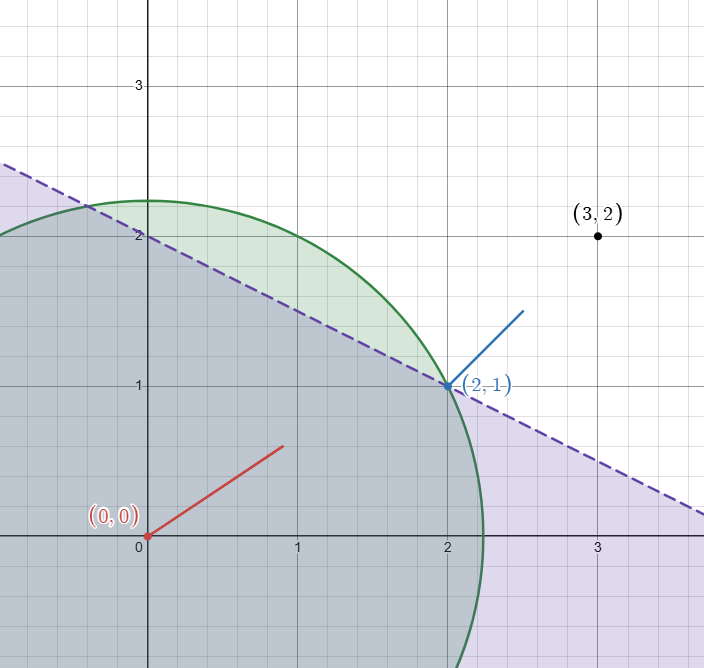
\includegraphics[width=0.6\textwidth]{pic/p7.png}
\end{figure}

\section{}
给定凸函数$f:R^n\rightarrow (−\infty,\infty]$, 向量$g$称为函数$f$在点$x$处的次梯度(subgradient),若满足\(f(z)\geq f(x) +g'(z −x),\forall z \in R^n\)。所有定义域上点的次梯度的集合称为次微分,记为$\partial f(x)$,试根据
这个定义求解下列函数的次微分集合,或者用图示的方式将次梯度的意义表示清楚:

\subsection{}
\[f(x) = |x|\]
\paragraph{解}
\[\partial f(x) = \left\{\begin{array}{cl}
  1 & x > 0\\
  -1 & x < 0\\
  \left[-1,1\right] & x = 0
\end{array}\right.\]

\subsection{}
\[f(x) = \max\{0,\frac{1}{2}(x^2 - 1)\}\]
\paragraph{解}
\[\partial f(x) = \left\{\begin{array}{cl}
  x & x < -1 \\
  \left[-1,0\right] & x = -1\\
  0 & -1 < x < 1\\
  \left[0,1\right] & x = 1\\
  x & x > 1
\end{array}\right.\]

\section{}
论述启发式优化算法的基本思想。点集匹配问题(给定两组特征点及其描述,如何确认其匹配的点)、拼图重构问题都是组合优化问题,如何采用启发式算法来求解? 

\paragraph{答}
启发式算法基本思想:在可接受的计算代价下找到最好的解,但不一定能保证解的最优性,是一种近似算法.通常是基于某种直观感觉或者经验构造的算法,在解决大规模,复杂的组合优化问题是有较好的表现。与最优化算法不同,启发式算法不需要提供一个最优解,而是提供一个在可接受精度范
围内的解,是精度和速度的权衡.

下面尝试给出点集匹配问题的启发式算法,首先形式化描述该问题,设点集$P$,$Q$分别是模板点集和目标点集,求映射\(f(p_i)=q_j,\forall p_i \in P\),目标函数通常定义为
\[g(P,Q)=\sum_{i,j \in P} d(p_i,p_j)-d(f(p_i)- f(p_j))+\lambda(n_P -n_{P'})\]

其中 \(f(p_i)\) 是目标点集的一个点,$p_i$ 是模板点集的一个点,$d(p_i,p_j)$ 是 P 中两个点的距离,$n_P,n_{P'},\lambda$ 分别是模板点集中的点总个数,模板点集中匹配上的点个数和惩罚系数.显然,惩罚系数越大,强迫找到一个该问题的最大匹配.

问题的难点在于如何得到映射f,考虑实际问题,可能是一个非线性的映射,如何建模该映射,以及如何找到一个最优的映射.

可以考虑用人工神经网络来建模该映射,直观上的理解神经网络是一个通用的函数拟合模型,对于神经网络参数的学习,可以通过引入模拟退火算法的随机梯度下降来获得一个较优的参数解. 可能存在的问题是有监督学习可能需要大量的样本对,对于图像的点集匹配问题,可以收集一定数量的图片,然后通过随机裁剪来获得样本对,尝试训练模型,得到问题的解.


\section{}
请给出几种求解大规模问题的分布式优化算法及其基本思想。 

\paragraph{答}
几种求解大规模问题的分布式优化算法:可以简单的将分布式优化算法按照有无中心节点分成两类:
\begin{itemize}
   \item 有中心节点算法基本思想是每个节点计算自身梯度,将信息传递给中心节点,中心节点汇聚所有节点信息后计算决策变量,然后将决策变量回传给各个子节点.
常见的有中心节点的分布式优化算法有ADMM,PSGD等,其优点是收敛速度快,但是缺点
是中心节点需要收集所有局部节点的信息有较大的延迟,中心节点需要较大的带宽,优化的过程也不够鲁棒.
    \item 无中心节点算法基本思想是每个节点计算自身梯度,然后将信息传递给邻居,每个节点通过自身和邻居节点的信息更新.常见的有分布式梯度下降算法DGD,其优点是通信负载均衡到每一个节点,鲁棒性和隐私性都好, 缺点是算法的设计需要单独考虑.
\end{itemize}


\section{}
论述罚因子方法与增广拉格朗日方法的基本思想,简述增广拉格朗日方法和ADMM方法的
异同。 
\paragraph{答}

罚因子方法: 将约束作为惩罚条件加入目标函数中,得到一个原约束问题的无约束辅助问题,利用无约束优化算法进行求解。主要有内点法和外点法两种形式。

\begin{itemize}
    \item 外点法:可以处理等式约束和不等式约束的情况,通过添加惩罚项,迫使迭代点向约束的可行域靠近。由于初始点的选取可以在约束可行域外随机选取,称为外点法。
    \item 内点法:只能处理不等式约束的情况,将惩罚添加在约束集边界。当可行解在约束界内,约束较小(可忽略);当解在约束界外,惩罚趋于无穷大,又称为闸函数法。需要注意的是,内点的初始点和迭代点需要在约束可行域内。
\end{itemize}

罚函数法通过构造辅助问题,将约束优化问题转换成无约束优化问题求解。但是,辅助问题的最优解想要达到对原问题解的较好近似,常常需要罚因子趋于无穷,此时出现了 $0^* \infty$ 的情况,可能会导致较大误差,实际求解变得很不方便。

增广拉格朗日方法的基本思想是通过将约束条件作为惩罚项加入拉格朗日函数,得到增广的拉格朗日函数。这种做法的好处在于利用了拉格朗日函数在 KKT 点导数为零的稳定性条件,克服了罚函数法中因为 $\nabla f(x) = 0$ 而出现的困难。同时,相比于拉格朗日法,增广后的方法也有明显的好处,即不再需要交替求解原始问题和对偶问题的解。同时,算法的速度和稳定性也有很大的提升,不再依赖每次搜索的步长。实际上,增广拉格朗日方法通过收敛性定理保证了对于大多数惩罚因子 $c$ 都有良好的收敛性,并且仅需关注求解对偶问题的解,即可通过解优化问题得到原始问题的解。

\section{}
思考:将非凸问题转化为凸问题有哪些可能的方法。 

\paragraph{答}

首先需要说明相比于非凸问题,凸问题的优势。对于凸问题,局部最优解就是全局最优解(更准确的说法是严格凸函数),同时,非凸问题的困难在于在高维空间中,存在许多鞍点(梯度为零,但是Hessian 矩阵不定)。

回顾凸问题的定义,需要满足两个条件(1)问题的可行域是一个凸集(2)目标函数是可行域上的一个凸函数。

在非凸问题转化成凸问题的过程中可以从这两个方向入手:
\begin{itemize}
   \item 修改目标函数,使其成为一个凸函数,这样就可以满足条件(1)。
   \item 抛弃一些约束条件,或者对约束条件做松弛处理,是的新的可行域是凸集,同时包含原可行域的所有点
\end{itemize}

\end{document}

